\documentclass[12pt, twocolumn]{article}
\usepackage{lmodern}

\usepackage{graphicx}
\usepackage{adjustbox}
\usepackage{tabularx}
\usepackage{subcaption}
\usepackage{minted}
%\usepackage{authblk}
% \usepackage{markdown}
% \usepackage[]{appendix}
\usepackage{amsmath}
\usepackage[printonlyused, nohyperlinks]{acronym}
\usepackage{amssymb}
\usepackage{listings}
\usepackage{booktabs}
% \input{snippets/tikz.tex}
% \usepackage[authoryear]{natbib}
\usepackage{float}
\usepackage{glossaries}
%\usepackage[hyphens]{url}
%\usepackage[german]{babel}
\usepackage[british]{babel}
\usepackage[utf8]{inputenc} %für Umlaute äüöß
\usepackage{array}
\usepackage[bookmarks]{hyperref}
\graphicspath{{img/}}
\usepackage{lmodern}
%avoid breaking across pages
\interfootnotelinepenalty=10000
\usepackage{xcolor}
\usepackage{multirow}
\usepackage{multicol}
\usepackage{tabu}
\usepackage{colortbl}
\usepackage{lipsum}

\newcommand{\RomanNumeralCaps}[1]
    {\MakeUppercase{\romannumeral #1}}


%adapting the article class to Ketter requirements
%\usepackage{showframe}
%\usepackage{setspace}
%\onehalfspacing
%\lstset{
%    basicstyle=\footnotesize,        % the size of the fonts that are used for the code
%    breakatwhitespace=false,         % sets if automatic breaks should only happen at whitespace
%    breaklines=true,                 % sets automatic line breaking
%    captionpos=b,                    % sets the caption-position to bottom
%    % deletekeywords={...},            % if you want to delete keywords from the given language
%    % escapeinside={\%*}{*)},          % if you want to add LaTeX within your code
%    % frame=single,                    % adds a frame around the code
%    keepspaces=true,                 % keeps spaces in text, useful for keeping indentation of code (possibly needs columns=flexible)
%    %  keywordstyle=\color{blue},       % keyword style
%    numbers=left,                    % where to put the line-numbers; possible values are (none, left, right)
%    numbersep=5pt,                   % how far the line-numbers are from the code
%    rulecolor=\color{black},         % if not set, the frame-color may be changed on line-breaks within not-black text (e.g. comments (green here))
%    showspaces=false,                % show spaces everywhere adding particular underscores; it overrides 'showstringspaces'
%    showstringspaces=false,          % underline spaces within strings only
%    showtabs=false,                  % show tabs within strings adding particular underscores
%    stepnumber=1,                    % the step between two line-numbers. If it's 1, each line will be numbered
%    tabsize=2,                       % sets default tabsize to 2 spaces
%}

%\makeglossaries
%\printglossaries

\newglossaryentry{economiccontrol}
{
	name=Economic Control,
	description={Control by the broker over customers regulatable devices such as storage devices or production devices}
}

\newglossaryentry{balancingcontrol}
{
	name=Balancing Control,
	description={Control which is managed by the \ac{DU} and performs the same as \gls{economiccontrol} activities.}
}




\usepackage{easylist}
\usepackage{hanging}
\usepackage{hyperref}
\usepackage{blindtext}
\usepackage{tipa}
\usepackage[left=2cm, top=2cm, bottom=2cm, right=1cm]{geometry}

\begin{document}

\begin{titlepage}

\begin{center}

\Huge{What methods should a trade uniion adopt to achieve its objectives?}
\vspace{10mm}

\normalsize{\today}


\vspace{10mm}


\begin{figure}[!h]
    \centering
    
\includegraphics[width=0.5\textwidth]{logo.png}
\end{figure}

\vspace{5mm}

\small{Industrial Managment\\ ECE -1}
\vspace{5mm}
\small{Department of Electronics and Communication And Engineering\\ Bharati Vidyapeeth College Of Engineering\\ }


\begin{multicols}{2}
\small{Ashish Arora - 01511502818} \\
\small{Ashwin Goyal - 01711502818} \\
\small{Bhavesh Dangwal - 01811502818} \\
\small{Bhupesh Bhatt - 01911502818} \\
\small{Deepanshu Tyagi - 02011502818} \\
\small{Divyanshu Bist - 02211502818} \\
\small{Ekansh Bhatnagar - 02311502818} \\
\small{Eshan Singh - 02411502818} \\
\small{Gagan Gupta - 02511502818} \\
\small{Gautam Manocha - 02611502818} \\
\end{multicols}

\end{center}

\end{titlepage}

\pagenumbering{Roman}

\onecolumn
\setcounter{tocdepth}{3}
\tableofcontents{}
\newpage


\twocolumn[

\begin{@twocolumnfalse}
\begin{abstract}
	Effective communication has been the backbone of strong relationships,
be it political, corporate or any other field. It is the first step in
forging ways that lead to trustworthy client relationships. Its
importance has been amplified by the current scenario. The corporate
world is on the precipice of change in the way it handles and manages
situations and also what they stand for. Therefore, effective
communication skills are becoming a must, more than they are already.

Focussing on a few of these skills viz. pronunciation, phonemic
awareness and fine motor skills, it is intended to identify the
different aspects of it, along with the concerns and problems that
people face in these areas. Also, ways to overcome these problems are
examined in order to be a better communicator.
\end{abstract}

\end{@twocolumnfalse}
]
\pagenumbering{arabic}
\section{Pronunciation Difficulties}

"Pronunciation" refers to the way in which we make the sound of words.
To pronounce words, we push air from our lungs up through our throat and vocal chords, through our mouth, past our tongue and out between our teeth and lips.
But there are some time when we might not be able to pronounce the words in the exact way in which they must be spelled

\begin{enumerate}
	\item  Stressing individual words incorrectly

If you usually speak with native English speakers, this will be the number one reason why they misunderstand you. It’s very hard for native English speakers to ‘translate’ a word spoken as ‘caLENdar’ to the way they would pronounce it, ‘CALendar’.  Non-native English speakers don’t have as much of a problem with this, and will probably still understand what you’re trying to say.

	\item Stressing the wrong words in a sentence.

		Remember that you can completely change the meaning of a sentence by stressing different words in that sentence. For example, you could say this sentence in a number of different ways:
		“I didn’t say we should drive this way.”
		If you stress I, you emphasize that taking that route wasn’t your idea. On the other hand, if you stress drive, you emphasize the mode of transport.
		If you don’t pay close attention to the words that you stress, you could end up sending a completely different message than the one you intended.


	\item Pronouncing certain consonant sounds incorrectly

If people are misunderstanding you, it could very well be due to you confusing what we call ‘voiced’ and ‘unvoiced’ sounds. You might substitute ‘p’ for ‘b’ or ‘t’ for ‘d’, for example. These sounds are so easily confused because their only difference is whether or not you use your voice to produce them. If you aren’t careful, you could be making mistakes like saying ‘tuck’ for ‘duck’ or ‘pay’ for ‘bay’.

	\item  Mixing up short and long vowel sounds

Vowel sounds, like consonant sounds, can also be confused easily. The main problem with vowels happens when you mix up long and short vowel sounds. For example, the long ‘ee’ sound in ‘seat’ with the short ‘i’ sound in ‘sit.’ If you confuse these sounds, you end up saying completely different words. This can get confusing in conversation and forces people to draw much more from the context of your speech than the speech itself.

	\item Forgetting to finish your words

Do you have a tendency to let your word endings drop? I often hear people drop the ‘ed’ ending off of words in the past tense, for example. This is a dangerous mistake because not only is your pronunciation wrong, but it also sounds like you’re making a grammatical mistake. People could judge you based on this type of error.

\end{enumerate}

\subsection{Types of difficulites faced in different environments and
situations}

Learning English Pronunications is very important for all professionals
in today's market. Good pronunicaiton makes a professional a good orator
which in turn helps on ones carreer. But certain difficulites in
pronunications can make a huge impact on a person's confidence. Research
shows the people with English as a second language have been noticed to
have much more difficulites that hinder the learning process in terms of
profiency in the oral and auditory skills. Many research papers have
also shown that phonetic difficulites affects older, but not younger,
speakers who stutter and that older speakers excpirence more difficulty
on content words thatn function words.

\subsubsection{Voiced Alveolar Approximant Sound}

The first four of the six wordsshown below demonstrate the use of the
turned R or voiced alveolar approximant sound in their pronunciation.
Represented by letter r, this sound in English can be seen in redor
zero. The pronunciation of the last two in the table, however, is some
how different from the first four. Being at the end of the words factor
and car, the voiced alveolar approximant sound becomes less stressed in
English.From the data analysed by the researchers, it was found out that
the students pronounced the letter ras voiced alveolar trill /r/. As the
researcherswere observing the presentations delivered bythe students,
thevoiced alveolar approximant sound,looked more like that of Indonesian
voiced alveolar trill sound.

\begin{figure}[h!]
	\centering
	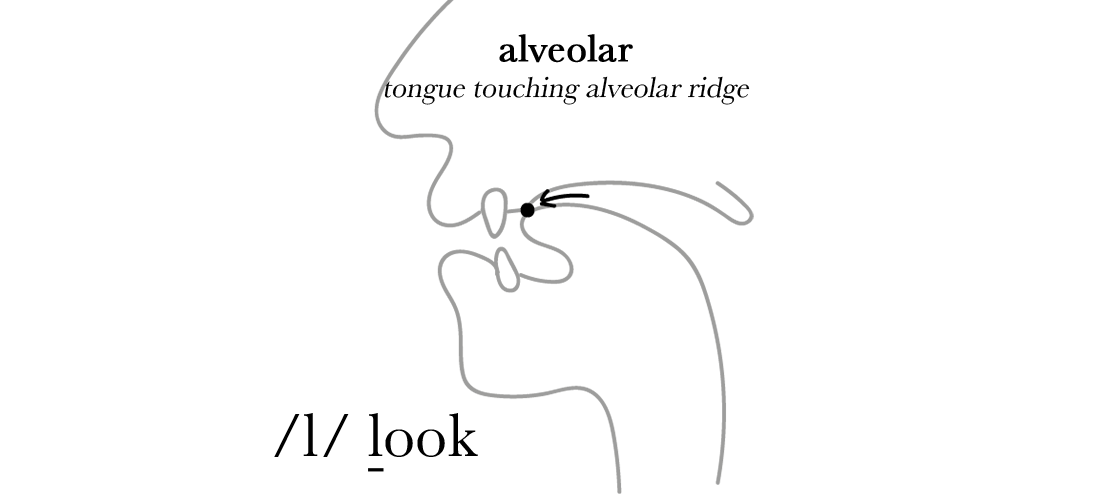
\includegraphics[scale=0.25]{img/lateral-approximant-mouth-position.png}
	\caption{Voiced Alveolar Approximant Sound}
	\label{fig:world}
\end{figure}

\subsubsection{Voiced Dental Fricative
Sound}

The data found and analysed by the researchers showed that the learners
also had problems with voiced dental fricative sound \dh. For this
sound, among other variations that appeared in the data,there are two
common pronunciationerrors they made. The first type of mistakethey made
is by assuming that the sound \dh/ is pronounced like voiced alveolar
plosive sound /d/. Other kinds of mistakes are also seen from the data.
They can be seen from how the students pronounced the worlds
/textit\{although\} and /textit\{brother\} and compared them to the
standard pronunicaiton of the given words. In additon, they also made
mistakes in treating other consonant and vowel sounds.

\begin{figure}[h!]
	\centering
	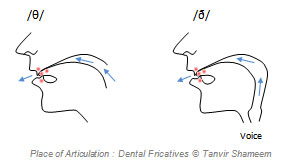
\includegraphics[scale=0.35]{img/dental.jpg}
	\caption{Voiced Dental Fricative Sound}
	\label{fig:world}
\end{figure}

\subsubsection{Voiceless Dental Fricative
Sound}

Still about dental fricative sounds, the students also found it
difficult to produce the voiceless type of the sound. Compared to the
previous kind discussed above, this sound is much more difficult for
them.This is seen from the interview done and from the fact that they
sometimes made it right in pronouncing voiced dental fricative sound
butthey hardly made it right when articulating the voiceless dental
fricative sound. Just like in the data presenting voiced dental
fricative sounds, the students also make mistakes related to sounds
other than voiceless dental fricatives.

\begin{figure}[h!]
	\centering
	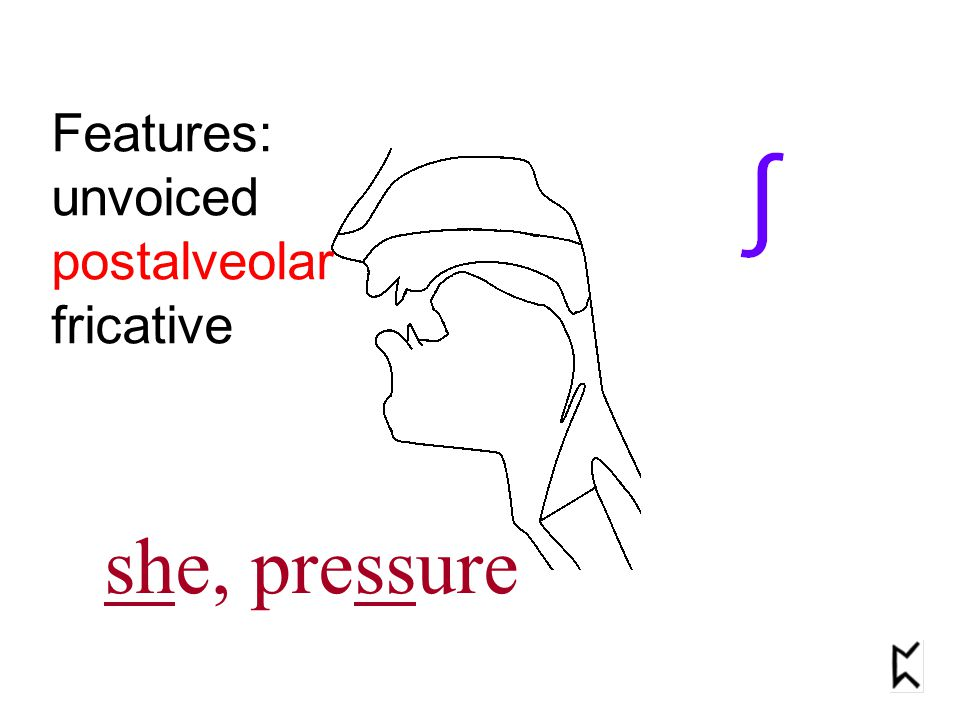
\includegraphics[scale=0.25]{img/post_alveolar.jpg}
	\caption{Voiceless Post-alveolar Fricative Sound}
	\label{fig:world}
\end{figure}
\subsubsection{Vocieless Post-alveolar Fricative
Sound}

The last common mistakes made by the students related to phonological
issues of consonantsis about voiceless post-alveolar fricative sound. In
English, this sound is represented by the combination of letters sand
hin succession. It is obvious from the data reported that this and other
kinds of phonological errors are potential to cause misunderstanding
from the listeners. The pronunications /si/ and /wcs/, might be
misunderstod as they sound more like see or sea and was rather sound
like she and wash as the actual words being used. Problems with this
voiceless post-alveolar fricative sound always occur whenever the
students found s and h being grouped and pronuncaed together.




\subsection{How to overcome Pronunciation Difficulties}

Overcoming the pronunciation barriers:

\begin{itemize}

\item One Phoneme at a time

While "improving pronunciation" as a goal might seem unattainable,
helping your students improve their pronunciation one phoneme at a time
is much more doable. Instead of taking up most of class time practicing
pronunciation, practice a different phoneme every day, or every week.

\item Practice the \textbf{Schwa}

The schwa sound [\textschwa] is the neutral vowel sound that typically occurs
in unstressed syllables, for example in words like choc(o)late, sep(a)rate, cam(e)ra, 
elab(o)rate, etc.  There are languages that pronounce these syllables differently
and students might be tempted to pronounce them as they do in their native tongue (this is
usually the case with Spanish speakers, where the central o in
"chocolate" is pronounced clearly). Teach students to be aware of
the [schwa sound] and learn to identify it as it will be tremendously useful in improving their
pronunciation.

\item Same Spelling Different Sounds

Students should learn that the same consonant combination may
have different sounds, for example the ch in chicken and character. The
sound [k] in character, in fact, may be spelled with a k, ck, c, ch or
que. The th combination is another example: it is pronounced [$\delta$]
in this, that, these, those; but it is pronounced [$\theta$]
in thin, thank, think, theory, for example. The gh combination is yet
another example, as it pronounced as a g (ghost) or f (rough). Practice
each of these combos and others one at a time.

\item Use Visuals

It's hard for students to simply imagine the difference in spelling, not
to mention remember all the different phonetic symbols; try to use
visual aids like [consonants flashcards] or [IPA
flashcards]. Use them for introduction and practice, and make sure students become familiar
with the symbols.

\item Learn to use the dictionary

You won't always be around to tell a student how a word is pronounced.
Teach them where to find the pronunciation for a word in the dictionary.
The best tool in this case is a [dictionary
app] with
sound, so that the student can hear the pronunciation with a simple
click. These tools help students become more independent and more
responsible for improving their pronunciation.

\end{itemize}




\section{Phonemic Awareness}

\subsection{What is phonemic awareness and what is its significance}

Ans: Phonemic awareness is the ability to hear and manipulate the sounds
in spoken words and the understanding that spoken words and syllables
are made up of sequences of speech sounds ,essential to learning to read
in an alphabetic writing system, because letters represent sounds or
phonemes. Without phonemic awareness, phonics makes little sense
Fundamental to mapping speech to print. If a child cannot hear that
/man/ and /moon/ begin with the same sound or cannot blend the
sounds /rrrrrruuuuuunnnnn/ into the word /run/, he or she may have
great difficulty connecting sounds with their written symbols or
blending sounds to make a word. Essential to learning to read in an
alphabetic writing system. A strong predictor of children who experience
early reading success.

\textbf{Phonemic Awareness Significance:}

1.  It requires readers to notice how letters represent sounds. It
    primes readers for print.

2.  It gives readers a way to approach sounding out and reading new
    words.

3.  It helps readers understand the alphabetic principle (that the
    letters in words are systematically represented by sounds).

\subsection{Benefits of phonemic awareness}

Once you becomes phonemically aware, phonics comes much more naturally. From there, spelling words will become a lot easier — when you split words into sounds, you will know which letters make up a word.
Children starting elementary school with a high level of phonemic awareness become more confident readers, making the process of learning to read a lot easier and more fun — when they come across new words, they can sound them out using their phonemic abilities.
phonemic awareness improves our reading abilities.Various studies shows the benefits of benefit of phonemic awareness
and  hildren who perform phonemic awareness activities are able to read more accurately and made “more substantial” progress in reading. The increase in accuracy results in improvement of
comprehension.These chodrem who perform these activities showed a remarkable ability to read new words. They could read words they’d never read before.So,overall knowlege of language with increase with increase
in phonemic awareness



\subsection{How to develop phonemic awareness}

The development of phonemic awareness starts right from the moment in which we are born.We hear different sounds and try to know the meaning and try to replicate the sound.that how ,our journey starts. but it is important to have a formal training in phonemic which will further help us in reading and writing also.
We start by dividing the word in greater chunks rather than dividing into smaller individual alphabet at very begining.It is much easier to hear the bigger units of language versus the individual sounds in a word. For example, asking children to segment pencil into two-syllables, /pen/ /cil/, is an easier task when compared to segmenting the word pen into three individual sounds, /p/ /e/ /n/.
The largest unit of language is a word.  Instruction in phonological awareness begins at the word level when children learn that compound words can be blended, segmented, and manipulated. For example, we can blend the small words class – room together to the compound word classroom. Or the opposite, we can segment compound words into two separate words. We can say the whole word and take it apart into two smaller words:  raincoat, rain – coat.  We can also substitute one small word in a compound word. Say sunshine, change shine to glasses and the word is sunglasses.

Once students can blend, segment, and manipulate compound words, we narrow the unit of language they hear and do the same work with syllables. For example, we blend the three syllables /cal – en – dar/, to say the whole word calendar.  Students can segment a word into syllables: elbow can be segmented into /el/ – /bow/.  We can substitute a syllable in a word to make a new word: reading; change /read/ to /talk/ and the word is talking.

We can narrow the unit of language again when we focus on the onset and rime. Onset-rime is breaking apart a syllable. The onset of a word is all the sounds that come before the vowel and the rime is the vowel and all the sounds after. Students blend the onset and rime into a whole word or segment a spoken word into the onset and rime.

\begin{enumerate}
\item Phoneme Isolation-Phoneme isolation is a skill where students hear and isolate a sound at the beginning of a word, middle of a word, and end of a word, often referred to as initial, medial, and final sounds.The first sound in the word name is /n/.
The final sound in the word bark is /k/.
The medial or vowel sound in the word cup is /u/.

\item Blending (parts to whole)-Blending is a skill that directly correlates to phonic decoding. Students hear sounds spoken aloud and they blend the sounds to make a word. During instruction, the teacher provides the phonemes and the students blend the phonemes into a whole word.	/s/ /u/ /n/, sun,/b/ /r/ /ā/ /k/, break,/p/ /r/ /i/ /s/, price

\item Segment (whole to parts)-Segmenting is a skill that directly correlates to encoding or spelling. Students hear a whole word and they segment the word into all the individual sounds they hear. During instruction, a teacher would say a whole word and students segment the word into individual phonemes.	week, /w/ – /ē/ – /k/,fox, /f/- /o/ -/k/- /s/,swim, /s/ -/w/ -/i/-/m/

\item Phoneme Manipulation (Add, Delete, Substitute): Phoneme manipulation is practiced with adding a phoneme, deleting a phoneme, or substituting a phoneme in spoken words.	Adding an initial sound to make a word: Add /s/ to /-at/ and the word is sat
Deleting an initial sound from a word: Say cup.  Without /k/, what’s left is, /-up/.
Substituting an initial sound:  The word is top. Change /t/ to /m/and the word is, mop.

\end{enumerate}

\section{Motor Skills}

Fine motor skills are the ability to make movements using the small muscles in our hands and wrists. Kids rely on these skills to do key tasks in school and in everyday life.

What are fine motor skills?
We use fine motor skills to make small movements. These movements come so naturally to most people that we usually don’t think about them. Fine motor skills are complex, however. They involve the coordinated efforts of the brain and muscles, and they’re built on the gross motor skills that allow us to make bigger movements.
Fine motor skills aren’t specific learning skills like reading or math are. But they directly impact how well kids are able to learn and show what they know. For instance, kids need fine motor skills to circle an answer in a bubble on a test or write an essay or response.
Kids need to use fine motor skills to do many school-related tasks. These include:
Holding a crayon or pencil
Drawing pictures and writing neatly
Stacking blocks and stringing beads
Using scissors, rulers, and other tools
Kids also need fine motor skills to do daily tasks like getting dressed and brushing their teeth.

\begin{figure}[h!]
	\centering
	
\includegraphics[scale=0.15]{img/brain-fine-motor.jpg}
	\caption{Learning Fine Motor skills}
	\label{fig:world}
\end{figure}


\subsection{Improving Motor Skills}


\subsubsection{Steps to improve fine motor skills in children:}

\begin{enumerate}
\item  Play-doug
\item  Puzzles
\item  Drawing, colouring in and painting
\item  Using kitchen tongs or tweezers
\item  Cutting with scissors
\item Toys and Games : Many toys develop fine motor skills, including those for infants and toddlers. For school-aged children, board games with pieces and parts to pick up and move are ideal for developing these skills. For instance, Jenga is a strategy game using fine motor skills that focus on the pincher grip, which is used in writing.
\item Origami: Origami is a paper-folding art that builds skills and is a fun family craft. You can use construction, wrapping or other decorative papers to make fine motor skill building origami shapes.  Papercutting activities build skills and control and can be as simple or complex as you need. Beginners can start with cutting out paper chains
and progress to more complex projects.
\item Sewing. Kitchen Counter Chronicles.
\item Weaving. Hands On As We Grow.
\item Lacing. Journey into Unschooling.
\item Beading.
\item Balancing.
\item Spooning Marbles.
\item Paint with Water.
\item Trace with Water.

\end{enumerate}

\subsubsection{Steps to improve fine motor skills in adults:}

\begin{enumerate}
\item Nuts and bolts, lacing beads, using clothespins to pick up Pom poms to
paint or just sort, buttons, zippers, snaps, putting marbles or rubber
balls on golf tees, making small balls with putty or play doh, sorting
jewelry, squeezing water out of sponges or towels, using different types
of tongs to pick up small objects
\item  Drawing a picture graded by changing the size of the paper. Bring in
different materials stampers, finger paint, etc
\item  Folding clothes (wash cloths, socks), ADL board (button, zippers bra
hooks etc), opening containers (toothpaste, lotion), clothes pins,
rainbow rings for crossing midline, velcro board, keys and locks,
theraputty, digiflex, beading craft
\item  My bin of various empty grocery containers is my go-to for fine motor
control skills to open/close, and having patients reach for them in
cabinets/refrigerators/shelves of various heights is one of my favorite
gross motor control activities.
\item  I take them straight to the kitchen and do bathroom stuff! I get them
to open their make-up containers, shampoo/conditioner bottles, wearing
weights while organizing shelves in the bathroom and or kitchen...make
meatballs, bread, pies for meal prep...opening different containers of
milk, using the manual can opener. Sorting dry a bag of dry beans for
meal prep...decorating cookies and cupcakes.
\item  Theraband activities or squeezing a ball are some of my favorite fine
motor activities to work on. - Noreena Ishtiaq
\item  I had a patient who had a stroke that was a retired banker. I brought
in all sorts of coins/dollars he really enjoyed sorting them into
various piles, placing them in stacks, etc.
\item  One easy fine motor activity I really like is to take a piece of
paper and using one hand, make it into a ball, then spread it out flat.
\item  But Rachel Hall, had a suggestion to take it one step farther to
grade it by starting with the paper on table then raise it up once in
the hand so no "cheating."
\item  My patient cleaned a tray table of shaving cream and told me she
liked doing a functional task.
\item  Playing video games.
\item  Using squirt bottles for cleaning.
\item  Squeezing a rubber ball or tennis ball.
\item  Pushing the affected fingers against a mattress.
\item  Fanning the fingers.
\item  Making a fist and holding as long as possible.
\item  Bouncing and catching a ball.
\item Crumpling and uncrumpling paper.

\end{enumerate}

\subsection{Concerns related to fine motor skills}

\begin{itemize}
\item
  \textbf{Bilateral Integration:}~Using two hands together with one hand
  leading (e.g. opening a jar lid with hand while the other hand helps
  to by stabilising the jar).
\item
  \textbf{Crossing Mid-line:}~The ability to cross the imaginary line
  running from a child's nose to pelvis that divides the body into left
  and right sides.
\item
  \textbf{Hand and finger strength:}~An ability to exert force against
  resistance using the hands and fingers that allows the necessary
  muscle power for controlled movement.
\item
  \textbf{Hand eye coordination:}~The ability to process information
  received from the eyes to control, guide and direct the hands in the
  performance of a task such as handwriting.
\item
  \textbf{Hand Dominance:}~The consistent use of one (usually the same)
  hand for task performance which allows refined skills to develop.
\item
  \textbf{Hand division:}~Using just the thumb, index and middle finger
  for manipulation, leaving the fourth and little finger tucked into the
  palm not participating but providing stability for the other 3
  fingers.
\item
  \textbf{Object Manipulation:}~The ability to skilfully manipulate
  tools (such as the ability to hold and move pencils and scissors with
  control) and the controlled use of everyday tools such as a
  toothbrush, hairbrush, and cutlery.
\item
  \textbf{Body Awareness (Proprioception):}~Information that the brain
  receives from our muscles and joints to make us aware of our body
  position and body movement, so we can accurately control our
  movements.
\end{itemize}

\textbf{Ativities can help improve fine motor skills}

\begin{itemize}
\item
  \textbf{Threading and lacing:~}with a variety of sized laces and
  beads.
\item
  \textbf{Tongs or teabag squeezers:}~to pick up objects (e.g. put
  marbles down a marble maze).
\item
  \textbf{Manipulation games:}~such as `Pick up Sticks' and `Connect 4'.
\item
  \textbf{Play-doh:}~Using the fingers, not the hands as whole; working
  with the Play-doh up in the air, not flat on the table.
\item
  \textbf{Construction:}~that requires pushing and pulling with fingers
  (e.g. `Mobilo', `K'nex' or `Lego').
\item
  \textbf{Storing construction materials}~in jars with screw lids that
  need to be opened and closed as the materials are needed and when
  packed away.
\item
  \textbf{Craft:}~Make things using old boxes, egg cartons, wool, paper
  and sticky or masking tape.
\end{itemize}

\section{Conclusion}


Pronunciation difficulties were defined and assessed. The main reasons
were found to be stressing wrong words, mixing up short and long vowels,
not finishing your words etc. Along with this, different type of
difficulties faced in different situations and environments were
defined. Ways to improve this skill were proposed such as using visuals,
using dictionary, learning schwa, practising etc.

Phonemic awareness was defined and its significance was highlighted. It
primes the readers for print and makes it easier to understand sounds.
Ways to improve along with the benefits of this skill were proposed such
as phoneme isolation and blending.

Finally, motor skills were defined and the concerns related to it were
assessed. Finally, ways to improve motor skills were proposed separately
for children and adults.


%\section{Introduction}

%The spread of COVID19, the respiratory disease origination from coronavirus
%occurred in Wuhan, China, is on the rise and has shaken the world. The World
%Health Organization named the disease COVID-19 when the first case of this
%virus was reported.

%The Global spread of COVID19 has affected most countries and was defined as a
%pandemic by the WHO in March 2020.

%This paper tracks the spread of the novel coronavirus, also known as the
%COVID-19. COVID-19 is a contagious respiratory virus that first started in
%Wuhan December 2019. \cite{data_world}

%The two types of coronaviruses, named as, severe acute respiratory syndrome
%coronavirus and (MERS-COV) have affected more than
%20,000 people in past decade \cite{huang2020clinical}.

%The coronavirus can spread by various means.However some of the common means through which the infection can occur are:

%\begin{enumerate}
%	\item airborne or aerosol transmission
%	\item direct or indirect contact with another human
%	\item and lastly through droplet spray transmission
%\end{enumerate}
%However a person can protect himself from these transmission modes.Close contact can be avoided and a minimum distance of 1.8 metres should be maintained to avoid contact with a person as well as respiratory droplets.However for airborne transmission a minimum of 4 metre should be maintained to avoid contact.Symptoms of COVID 19 are coughing ,extreme fever,tiredness or weakness and pain in some joints of the body.

%%% Respiratory infections can be transmitted through droplets of different sizes:
%%when the droplet particles are $>5-10 \mu m$ in diameter they are referred to as respiratory droplets, and when then
%%are $<5 \mu m$ in diameter, they are referred to as droplet nuclei. According to current evidence, COVID-19 virus
%%is primarily transmitted between people through respiratory droplets and contact routes. In an analysis of
%%75,465 COVID-19 cases in China, airborne transmission was not reported. Droplet transmission occurs when
%%a person is in in close contact (within 1 m) with someone who has respiratory symptoms (e.g., coughing or
%%sneezing) and is therefore at risk of having his/her mucosae (mouth and nose) or conjunctiva (eyes) exposed
%%to potentially infective respiratory droplets. Symptoms as fever, cough, and shortness of breath after a period
%%ranging from 2 to 14 days are observed as the outcomes of the disease. Detailed investigations found that
%%SARS-CoV was transmitted from civet cats to humans in China in 2002 and MERS-CoV from dromedary
%%camels to humans in Saudi Arabia in 2012. Several known coronaviruses are circulating in animals that have
%%not yet infected humans.
%So for helping combat coronavirus machine learning and deep learning models are used in this paper.These model
%will gives us a rough estimate as to how the disease will spread in the upcoming days how many more people
%will be effected.It will a rough estimate to the government of various countries about how the spread and will
%enable them to be prepared well in advance for the epidemic.

%Most of the data driven approaches used in previous studies
%\cite{knight2016bridging} have been linear models and often neglects the
%temporal components of the data.


%In this report data preprocessing techniques are  applied on the confirmed cases data and then the preprocessed
%data is applied to two models i.e. LSTM and Linear Regression .The real and predicted cases are compared on
%a predefined metrics.A comparative study is drawn to see the performance of
%LSTM and Linear regression model to see which model best for the data.

%The section \textbf{Literature Review} talks about similar work done by
%other researchers on this topic and talk about the model and approach used by
%them.

%The methodology used in the paper and the approach on how to handle this
%problem is also discussed.

%The section \textbf{Methods and models} talks about the dataset used and and its
%features. Since classification is done worldwide, so the data was processed to
%suite the needs of the models in use and a brief description of the processed
%dataset was also provided.

%Next, Evaluation metrics are discussed to understand and compare the result
%between the two models used. MAPE and Accuracy were used to compare the result
%and were used to draw conclusions.

%Also the models of Linear regression and LSTM network are explained
%demonstrating our approach.

%In the end \textbf{Experiment Result} are shown. Evaluation metrics are used
%to compare the result.

%%\pagebreak

%\section{Literature Review}

%In \cite{hu2020artificial},an machine learning based alternative to
%transmission dynamics for Covid-19 is used. This AI based approach is executed by implementing modified stacked
%auto-encoder model.

%In \cite{bandyopadhyay2020machine}, an deep learning based approach is
%proposed to compared the predicted forecasting value of LSTM and GRU model. The
%Model was prepared and tested on the data and a comparison was made using the
%predefined metrics.

%In \cite{ayyoubzadeh2020predicting}, LSTM and Linear regression model was used
%to predict the COVID-19 incidence through Analysis of Google Trends data in
%Iran. The Model were compared on the Basis of RMSE metrics.

%In \cite{chimmula2020time}, an LSTM networks based approach is proposed for
%forecasting time series data of COVID\-19 in Canada.
%This paper uses LSTM network to overcome problems faced by linear model where
%algorithms assigns high probability and neglects temporal information leading to
%biased predictions.

%In \cite{fanelli2020analysis}, temporal dynamics of the corona virus outbreak
%in China, Italy, and France in the span of three months are analyzed.

%In \cite{bouktif2018optimal}, Several linear and non-linear machine learning algorithms were trained and
%picked the best one as baseline, after that chose the best features using wrapper and
%embedded feature selection methods and finally used genetic algorithm (GA) to find
%optimal time lags and number of layers for LSTM model predictive performance
%optimization.

%In \cite{yang2020modified}, temporal dynamics of the corona virus outbreak in China, Italy, and France in
%the span of three months are analysed.

%%In \cite{anastassopoulou2020data}, a computation and analysis based on Suspected-Infected-Recovered-Dead
%%(SIRD) model is provided. Based on the dataset, it estimates the parameters, i.e. the
%%basic reproduction number (R0) and the infection, recovery and mortality rates,

%In \cite{rainisch2020dynamic},a modeling tool was constructed to aid active public health officials to estimate
%healthcare demand from the pandemic.The model used was SEIR compartmental model
%to project the pandemic’s local spread.

%In \cite{singh2020connecting},a transmission network visualization (s) of COVID-19 in India was created and
%analysis was performed upon them. Using the transmission networks obtained there was
%an attempt to find the possible Super Spreader Individual (s) and Super Spreader Events
%(SSE) responsible for the outbreak in their respective regions.

%In \cite{elmousalami2020day}, it presents a comparison of day level forecasting models on COVID-19 affected
%cases using time series models and mathematical formulation. The forecasting models
%and data are used to suggest that the number of coronavirus cases grows exponentially
%in countries that do not mandate quarantines.

%In \cite{roosa2020real},phenomenological models that have been validated during previous outbreaks
%were used to generate and assess short-term forecasts of the cumulative number of
%confirmed reported cases in Hubei province.

%\subsection{Our Work}

%In our report, the confirmed cases of corona virus are studied from the start
%of the epidemic and the two approaches of Linear Regression and LSTM networks
%are used, and an report is presented stating which of the above stated model
%works best these type of data on the basis of Mean Absolute Error.

%\begin{figure}[h!]
%	\centering
%	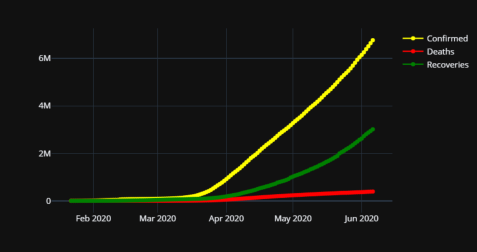
\includegraphics[scale=0.4]{img/world_wide.png}
%	\caption{Number of cases around the world}
%	\label{fig:world}
%\end{figure}

%%\section{Theory}
%%
%%

%%\pagebreak

%\section{Methods and models}

%\subsection{Data}
%The dataset used was the 2019 Novel Coronavirus Dataset operated by the
%Johns Hopkins University Center for Systems Science and Engineering
%(JHU CSSE).

%It consist of 3 dataset each of Death, Confirmed, Recovered cases of 188
%countries datewise. The number of date columns are 138 starting from 22
%Jan,2020 to 8 June,2020.Out of this about 85\% are used as training data
%and the rest used as testing and validating data. So the model would be
%predicting next 15\% data value.

%The prediction would not be made on a specific country rather it will be
%worldwide.

%\begin{table}[!ht]
%	\caption{World Dataset of Corona virus spread with confirmed, death,
%	and recovery rates}
%	\centering
%	\resizebox{\columnwidth}{1.5cm}{%
%		\begin{tabular}{lrrrrrrrr}
%			\toprule
%			{} &     Confirmed &    Recoveries &         Deaths &
%			Confirmed Change &  Recovery Rate &  Growth Rate & \\
%			\midrule
%			count &  1.390000e+02 &  1.390000e+02 &     139.000000 &        138.000000 &     139.000000 &   138.000000 \\
%			mean  &  1.918547e+06 &  6.817390e+05 &  123264.726619 &      50666.268116 &       0.286331 &     0.076081 \\
%			std   &  2.170725e+06 &  8.911273e+05 &  138597.907312 &      42526.463980 &       0.143922 &     0.117824 \\
%			min   &  5.400000e+02 &  2.800000e+01 &      17.000000 &         89.000000 &       0.017598 &     0.005032 \\
%			25\%   &  7.862450e+04 &  2.747150e+04 &    2703.000000 &       2957.500000 &       0.207790 &     0.021193 \\
%			50\%   &  8.430870e+05 &  1.738930e+05 &   44056.000000 &      67738.000000 &       0.288055 &     0.032183 \\
%			75\%   &  3.546736e+06 &  1.142438e+06 &  249918.000000 &      84446.500000 &       0.395898 &     0.085793 \\
%			max   &  6.992485e+06 &  3.220219e+06 &  397840.000000 &     130518.000000 &       0.544809 &     0.951446 \\
%			\bottomrule
%		\end{tabular}}
%	  \label{table:world_df}
%\end{table}

%Table [\ref{table:world_df}] show the world data of Corona virus spread with
%confirmed, death and recovery rates.

%%\pagebreak
%\subsection{Evaluation Metrics}

%To identify best model, it is necessary to put concentration on comparison of measures of
%the algorithm’s performance. In this report, MAPE and Accuracy are used to
%measure algorithm's performance-

%\begin{enumerate}
%	\item \textbf{Mean Absolute Percentage Error}: It is defined by
%		the following formula:
%		\begin{equation}\label{eqn1}
%			%E = {mc^2}
%			MAPE = \frac{100\%}{n} \sum \left \vert \frac{y-y\prime}{y}
%			\right \vert
%		\end{equation}

%		Where y is true value and y' is predicted value.

%	\item \textbf{Accuracy}: It is defined by the following formula:
%		\begin{equation}\label{eqn2}
%			Accuracy = (100 - MAPE)\%
%		\end{equation}

%\end{enumerate}


%\begin{figure*}[!ht]
%	  \centering
%	  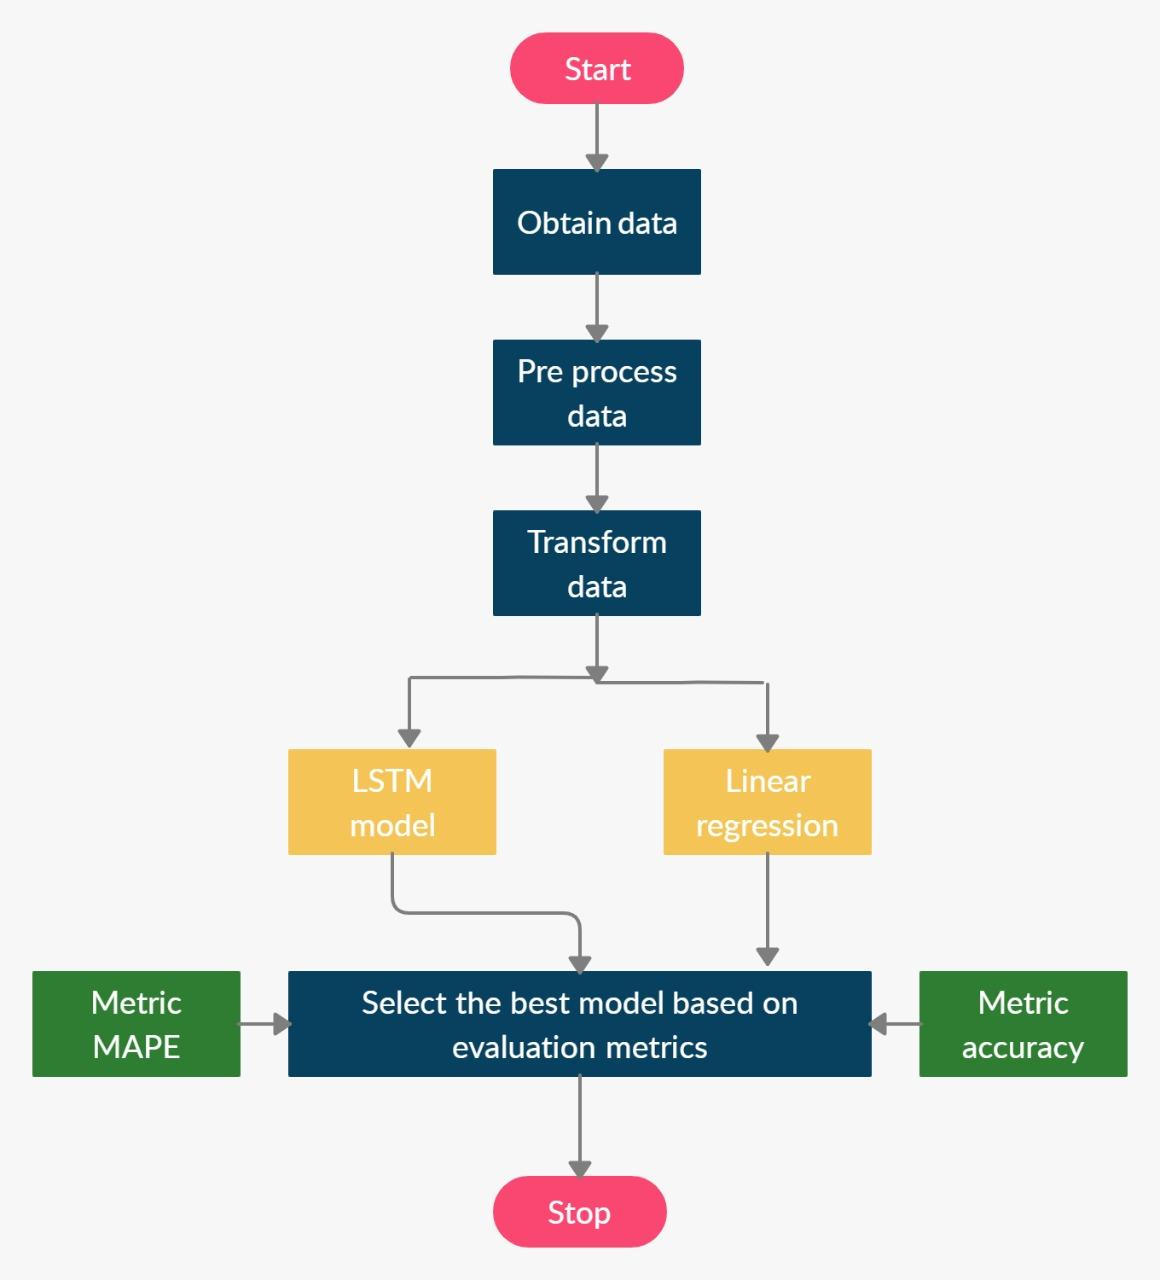
\includegraphics[height=14cm]{img/method.jpg}
%	  \caption{Flowchart for proposed methodology}
%	  \label{fig:method_flow}
%\end{figure*}

%\subsection{Method}

%The prediction of confirmed cases of COVID 19 Corona virus are obtained
%using a Recurrent Neural Network method(LSTM) and Linear Regression.

%Linear regression is a linear model, that assumes a linear relationship between the input variables
%(x) and the single output variable (y).When there is a single input variable (x), the method
%is referred to as simple linear regression.

%A Recurrent Neural Network (RNN) is kind of neural network architecture that considers
%both sequential and parallel information processing. Incorporating memory cells to neural
%network; it is possible to simulate the operations similar to human brain.There are
%alternatives from RNN depending on the gating units, such as Long Short Term Memory
%(LSTM) RNN and Gated Recurrent Unit (GRU) RNN.Traditional RNN lacks of
%considering context based prediction, which can be overcome by introducing Long short-
%term memory (LSTM). LSTM has a good potential to regulate gradient flow and enable
%better preservation of long-range dependencies \cite{bandyopadhyay2020machine}.

%The dataset used for predicting the value is taken from John Hopkin University which
%contains cases form 22 January 2020 to 8 June,2020.Training and testing of both the models
%is done on this dataset.It contains 138 date columns out of which 120 are used for training
%and the rest 18days are used for testing data or for forecasting it.At first the data is preprocessed by converting the date columns into datetime object and also eliminate the
%missing values. The preprocessed data is then transformed in the required shape to be put
%into the model.The models are trained and the test data is predicted and prediction result
%are quantified using performance measures metrics such as MAPE and
%accuracy.The methodology performed for each of the step is shown in the figure
%\ref{fig:method_flow} as show.

%\subsubsection{Linear Regression}
%Linear regression is used for prediction tasks.In a problem with one predicting value this
%technique is used which tries to best fit the value to a linear line.This line can be used to
%relate both the predicting and predicted value.When there is more than one value then the

%In case of exponential relations, linear regression can not be directly used.
%But after transformation to a linear expression, even exponential relations can
%be predicted using linear regression. For example,
%\begin{equation}
%	y = \alpha e^{\beta x}
%\end{equation}

%Taking the log on both sides of the equation, we get:

%\begin{equation}
%	\ln y = \ln \alpha + \beta x
%\end{equation}

%This expression is of the form of a linear regression model:
%\begin{equation}
%	y\prime = \alpha \prime + \beta x
%\end{equation}


%%\pagebreak

%\subsubsection{LSTM Model}

%Long Short term memory is an recurrent neural network which is most effective for time
%series prediction.The model used in this case is sequential.As the data was time series and
%we needed to predict the best positive corona cases so this model was best for our study.The
%model was build using tensorflow keras framework and the models performance was
%evaluated on the mean absolute error percentage (MAPE) and accuracy metrics.
%The proposed architecture of LSTM model is shown in the figure
%\ref{fig:lstm_arch} as:

%\begin{figure}[ht!]
%	\centering
%	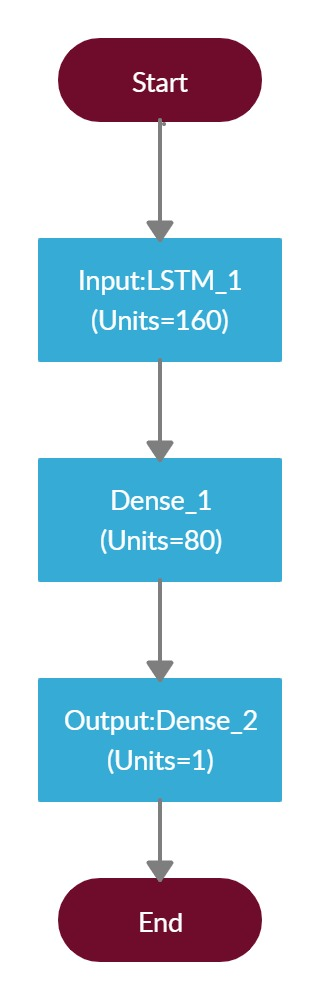
\includegraphics[scale=0.5]{img/lstm_mod.jpg}
%	\caption{Architecture of LSTM model}
%	\label{fig:lstm_arch}
%\end{figure}

%\newpage

%\section{Experiment Result}

%In LSTM model, LSTM layers use sequence of 180 nodes. A 1 layered structure followed by
%2 Dense Layers with 60 nodes in the first layer and 1 node in the output layer is used as LSTM model for verifying prediction result. The best
%hyperparameters used is a batch size of 1.The prediction accuracy of the model
%is shown in table \ref{table:lstm}

%\begin{table}[ht!]
%	\centering
%	\caption{Accuracy and MAPE of LSTM model}
%	\begin{tabular}{c c c}
%		Model & Accuracy & MAPE \\
%		LSTM model & 96.90\% & 3.092\%
%	\end{tabular}
%	\label{table:lstm}
%\end{table}

%%\pagebreak
%The prediction result is shown in figure below:
%\begin{figure}[ht!]
%	\centering
%	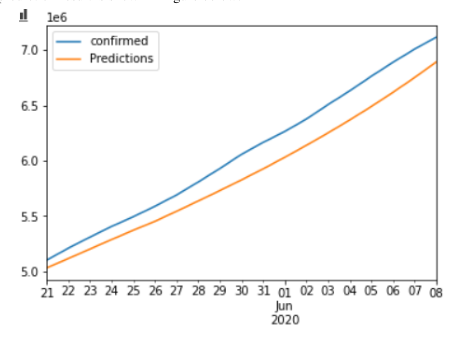
\includegraphics[scale=0.5]{img/lstm_graph.png}
%	\caption{Comparison of predicted and true value using LSTM model}
%	\label{fig:lstm_graph}
%\end{figure}
%%\pagebreak

%Linear regression was also applied on the time series data and the date columns were taken
%as input and the 18 days data was predicted. The exponential fit of the model
%was fit and the prediction accuracy of the model is shown in table
%\ref{table:linear}

%\begin{table}[ht!]
%	\centering
%	\caption{Accuracy and MAPE of regression model}
%	\begin{tabular}{c c c}
%		Model & Accuracy & MAPE \\
%		Linear model & 93.57\% & 6.421\%
%	\end{tabular}
%	\label{table:linear}
%\end{table}

%The prediction result of comparing the test data predicted data is show below:
%\begin{figure}[ht!]
%	\centering
%	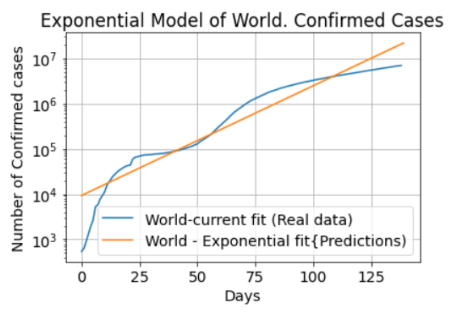
\includegraphics[scale=0.5]{img/linear_graph.png}
%	\caption{Comparison of predicted and true value using Linear Regression model}
%	\label{fig:linear_graph}
%\end{figure}

%\pagebreak

%\subsection{Comparing with other studies}
%%
%In \cite{hu2020artificial}, they used an multi-step forecasting system on
%the population of china, and the estimated average errors are as show in
%\ref{table:three}

%\begin{table}[ht!]
%	\centering
%	\caption{Result \cite{hu2020artificial}: Method and Average Errors}
%	\begin{tabular}{c c }
%		Model & Error  \\
%		6-Step & 1.64\% \\
%		7-Step & 2.27\% \\
%		8-Step & 2.14\% \\
%		9-Step & 2.08\% \\
%		10-Step & 0.73\%
%	\end{tabular}
%	\label{table:three}
%\end{table}


%In \cite{chimmula2020time}, LSTM netwoks are used to on Canadian population,
%the reuslt are show is table \ref{table:four}

%\begin{table}[ht!]
%	\centering
%	\caption{Results \cite{chimmula2020time}: Canadian Datasets}
%	\begin{tabular}{c c c}
%		Model & RMSE & Accuracy \\
%		LSTM & 34.63 & 93.4\%

%	\end{tabular}
%	\label{table:four}
%\end{table}


%In \cite{bandyopadhyay2020machine}, an deep learning based approach is
%proposed to compared the predicted forcasting value of LSTM and GRU model is
%used the result are as show in table \ref{table:seven}:

%\begin{table}[ht!]
%	\centering
%	\caption{Results \cite{chimmula2020time}: Canadian Datasets}
%	\begin{tabular}{c c c}
%		Model & RMSE & Accuracy \\
%		LSTM & 53.35 & 76.6\% \\
%		GRU & 30.95 & 76.9\% \\
%		LSTM and GRU & 30.15 & 87\%

%	\end{tabular}
%	\label{table:seven}
%\end{table}

%\section{Conclusion and Future Scope}

%The comparison between Regression and LSTM model signifies that LSTM provides a
%comparatively better results in terms of prediction of confirmed data. This paper showcases a method that checks occurred cases of
%COVID-19. However it could be made automated to train on the updated data
%every week and see the predicted value. Also the model is trained only on confirmed cases
%same could be done for both recovered and death cases and predicted values could be found.
%The model shows only the worldwide cases however the dataset also provides country wise
%statistics so it can be used by different country to forecast the future outcome of the
%pandemic and take necessary preventive measures to be safe from this worldwide
%pandemic.  In conclusion,
%the data mining models could help policymakers and health managers to plan health care
%resources and control the prevention of an epidemic outbreak. The availability of high-
%quality and timely data in the early stages of the outbreak collaboration of
%the researchers to analyze the data could have positive effects on health care
%resource planning.

%%\newpage



% \nocite{*}
% % %Bibliogra*phy
%  \addcontentsline{toc}{section}{Bibliography}
%  \bibliographystyle{apalike}
%  \bibliography{bibliography}

\end{document}
